% arara: pdflatex: { shell: yes }
\documentclass[twoside]{article}
\usepackage[utf8]{inputenc}
\usepackage[english]{babel}
\usepackage{amsmath, amssymb, amsthm}
\usepackage{hyperref}
\usepackage{ragged2e}
\usepackage{graphicx}
\usepackage{float}
\usepackage{fancyhdr}
\usepackage{geometry}
\usepackage{multicol}
\usepackage{url}
\usepackage{listings} % For better code formatting
\usepackage{xcolor} % For syntax highlighting

% Suppress underfull and overfull warnings
\tolerance=1000
\emergencystretch=10pt

\setlength{\headheight}{15.2pt}
\geometry{paperwidth=8.5in, paperheight=11.0in, top=1.0in, bottom=1.0in, left=1.0in, right=1.0in}

\pagestyle{fancyplain}
\fancyhead[LO]{Activity \#2.1}
\fancyhead[CO]{}
\fancyhead[RO]{P25-LIS-3012}
\fancyfoot[LO]{\thepage}
\fancyfoot[CO]{Advanced Databases, UDLAP}
\fancyfoot[RO]{}

% Define a style for XQuery code
\lstdefinestyle{xquery}{
	basicstyle=\ttfamily\small,
	breaklines=true, % Allow line breaks
	breakatwhitespace=true, % Break lines at spaces
	frame=single, % Add a frame around the code
	captionpos=b, % Caption position
	keywordstyle=\color{blue}, % Keywords in blue
	commentstyle=\color{green}, % Comments in green
	stringstyle=\color{red}, % Strings in red
	numbers=left, % Line numbers on the left
	numberstyle=\tiny\color{gray}, % Line numbers style
	tabsize=2, % Tab size
	showstringspaces=false % Don't show spaces in strings
}

\begin{document}

\fancypagestyle{plain}{
	\renewcommand{\headrulewidth}{1pt}
	\renewcommand{\footrulewidth}{1pt}
}

\title{XQuery Language}
\author{\small{Erick Gonzalez Parada ID: 178145}\\
	\small{Emiliano Ruiz Plancarte ID: 177478} \\
	\small{Andre Francois Duhamel Gutierrez ID: 177315} \\
\small{Antonio Gutiérrez Blanco ID: 177442}}
\date{\today}
\maketitle

\begin{abstract}
	\raggedright
	This document explores the fundamentals of the XQuery language, showcasing query examples, methodologies, and conclusions drawn from practical applications.
\end{abstract}

\begin{justify}
	\textbf{\textit{Keywords:}} XML, DTD, XPath, XQuery, BaseX.
\end{justify}

\section{Theoretical Framework}
XQuery is a powerful and flexible query language designed for querying and transforming XML data. It is often referred to as "SQL for XML" due to its ability to extract and manipulate data stored in XML documents. XQuery is built on XPath expressions and provides additional features such as FLWOR (For, Let, Where, Order by, Return) expressions, which allow for complex data retrieval and transformation tasks \cite{w3}.

One of the key strengths of XQuery is its ability to handle hierarchical and nested data structures, which are common in XML documents. This makes it particularly useful for applications such as web services, data integration, and content management systems. For example, XQuery can be used to extract specific elements from an XML document, transform the data into a different format, or generate reports based on the data \cite{microsoft}.

Another important feature of XQuery is its support for strong typing and schema validation. This ensures that the data being queried adheres to a predefined structure, reducing the risk of errors and improving the reliability of the queries. Additionally, XQuery supports modularity, allowing developers to create reusable modules and functions that can be shared across different projects \cite{w3schools}.

\subsection*{Goals}
The goal of this lab is to have a first encounter with the XQuery language to examine XML
documents.

\subsection*{Materials}
\begin{itemize}
	\item \textit{BaseX}
\end{itemize}

\section{Methodology}
The methodology involves writing and executing XQuery scripts to perform the operations on the XML documents. Each query is designed to demonstrate a specific feature or use case of XQuery, such as filtering, sorting, grouping, and transforming data. The results of each query are analyzed to understand the underlying principles and techniques.

\section{Query Results}
Below are the XQuery scripts and their corresponding results:

Here is the corrected chunk of LaTeX with added captions and explanations for each figure:


\begin{enumerate}
%1
	\item List books published by "Addison-Wesley" after 1991:
		\begin{lstlisting}[style=xquery]
			let $books := doc("bookshop.xml")//book
			where $books/publisher = "Addison-Wesley" and $books/@year > 1991
			return <book><year>{$books/@year}</year><title>{$books/title/text()}</title></book>
		\end{lstlisting}
		\subsection*{Query Result}
		\begin{figure}[H]
			\centering
			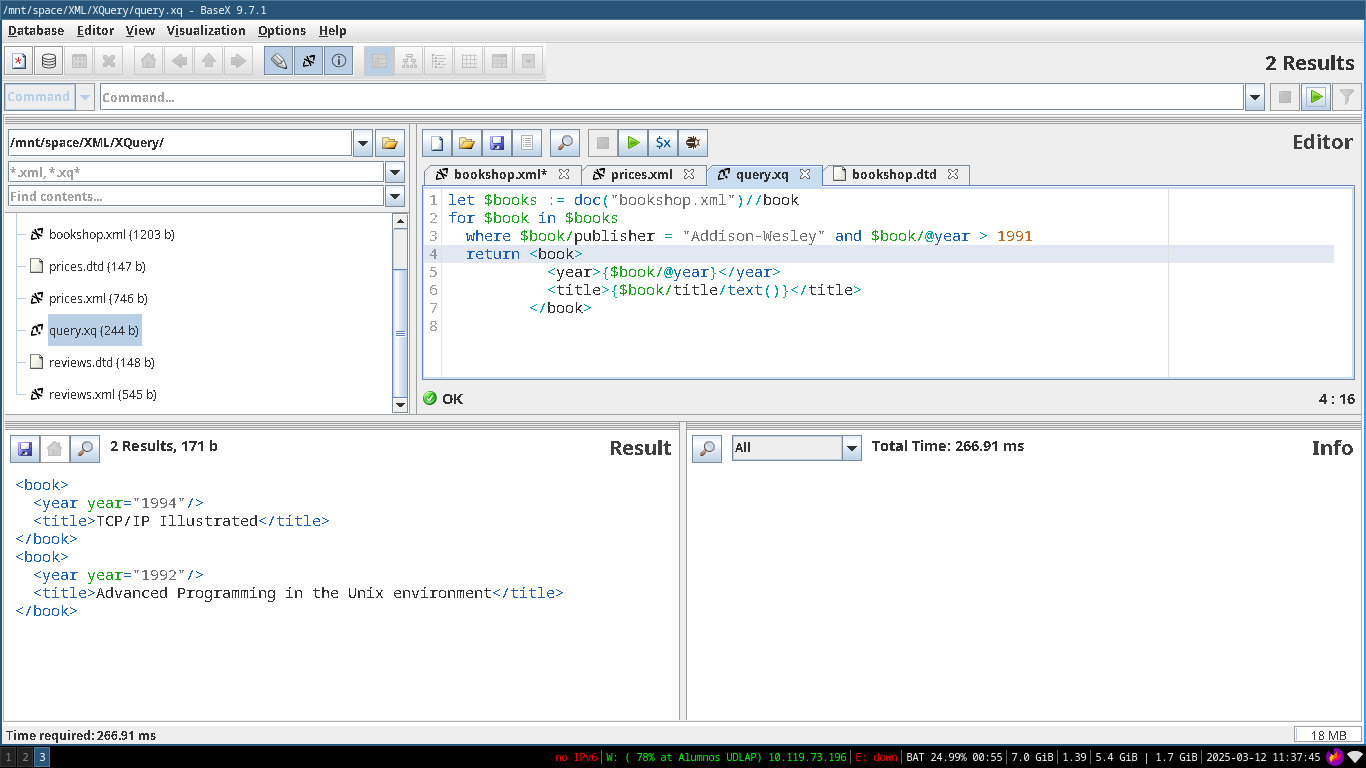
\includegraphics[width=1\textwidth]{imgs/x1.jpeg}
			\caption{Books published by Addison-Wesley after 1991.}
			\label{fig:1}
			\small{The query filters books by publisher and year, returning the year and title of each book.}
		\end{figure}
%2
	\item Create a flattened list of "result" items with title and author:
		\begin{lstlisting}[style=xquery]
			for $book in doc("bookshop.xml")//book,
			$author in $book/author
			return <result><title>{$book/title/text()}</title><author>{$author/name/text()} {$author/lastname/text()}</author></result>
		\end{lstlisting}
		\subsection*{Query Result}
		\begin{figure}[H]
			\centering
			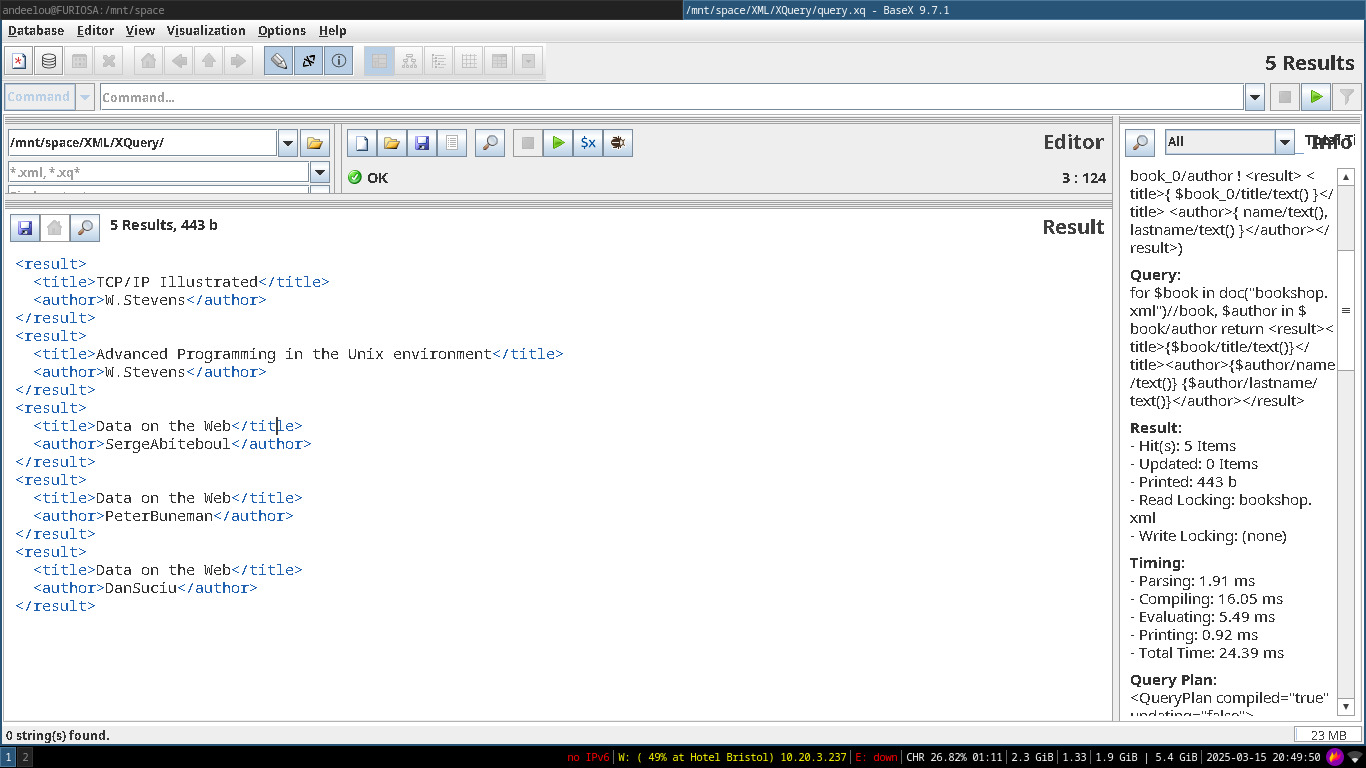
\includegraphics[width=1\textwidth]{imgs/x2.jpeg}
			\caption{Flattened list of books with titles and authors.}
			\label{fig:2}
			\small{The query iterates over each book and author, creating a flat list of results with titles and authors.}
		\end{figure}
%3
	\item List titles with grouped authors:
		\begin{lstlisting}[style=xquery]
			for $book in doc("bookshop.xml")//book
			return <result>
			<title>{$book/title/text()}</title>
			<authors>{
				for $author in $book/author
				return <author>{$author/name/text()} {$author/lastname/text()}</author>
			}</authors>
			</result>
		\end{lstlisting}
		\subsection*{Query Result}
		\begin{figure}[H]
			\centering
			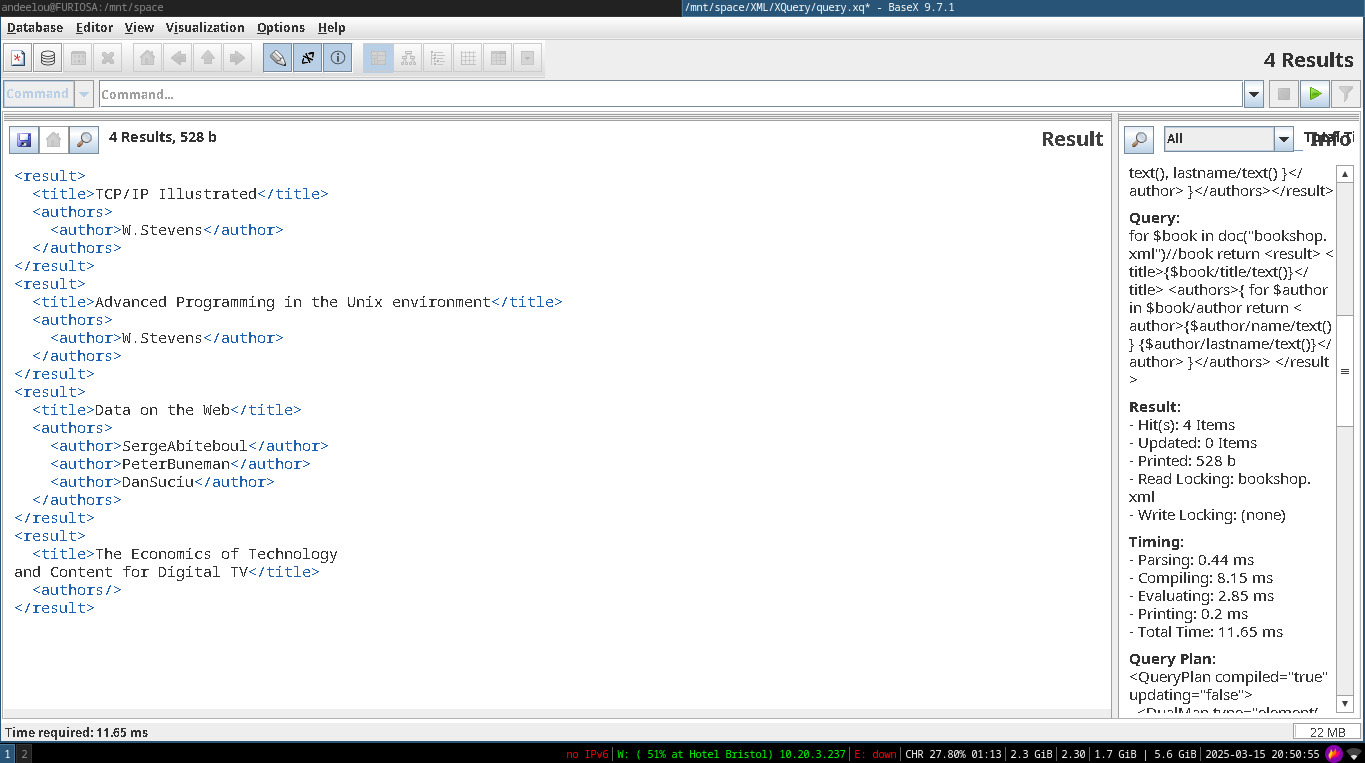
\includegraphics[width=1\textwidth]{imgs/x3.jpeg}
			\caption{Book titles with grouped authors.}
			\label{fig:3}
			\small{The query groups authors under each book title, creating a nested structure.}
		\end{figure}
%4
	\item List authors with their books:
		\begin{lstlisting}[style=xquery]
			for $author in distinct-values(doc("bookshop.xml")//author)
			let $books := doc("bookshop.xml")//book[author/name = $author/name and author/lastname = $author/lastname]
			return <result>
			<author>{$author/name/text()} {$author/lastname/text()}</author>
			<titles>{
				for $book in $books
				return <title>{$book/title/text()}</title>
			}</titles>
			</result>
		\end{lstlisting}
		\subsection*{Query Result}
		\begin{figure}[H]
			\centering
			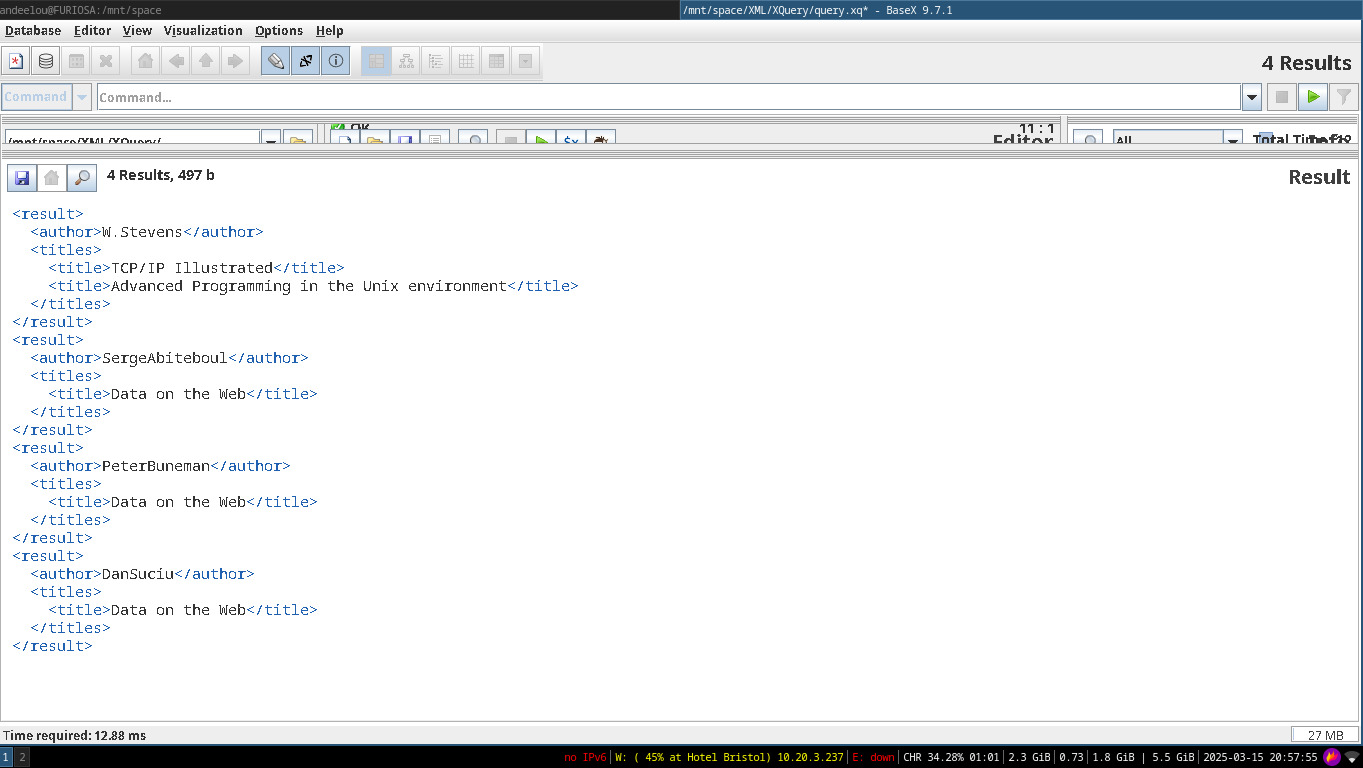
\includegraphics[width=1\textwidth]{imgs/x4.jpeg}
			\caption{Authors with their corresponding books.}
			\label{fig:4}
			\small{The query lists each author along with the titles of their books.}
		\end{figure}
%5
	\item Books with number of authors:
		\begin{lstlisting}[style=xquery]
			for $book in doc("bookshop.xml")//book
			return <book>
			<title>{$book/title/text()}</title>
			{if ($book/author) then <number-of-authors>{count($book/author)}</number-of-authors> else ()}
			</book>
		\end{lstlisting}
		\subsection*{Query Result}
		\begin{figure}[H]
			\centering
			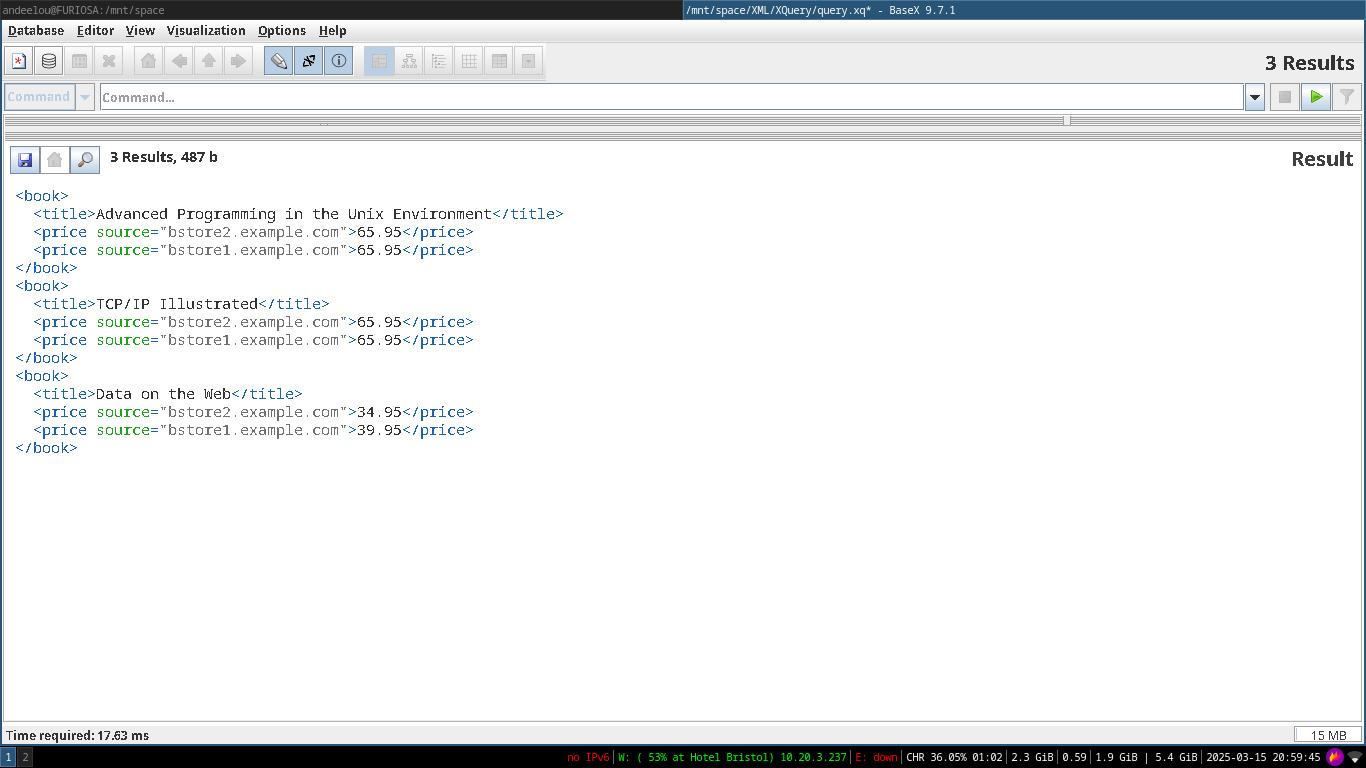
\includegraphics[width=1\textwidth]{imgs/x5.jpeg}
			\caption{Books with the number of authors.}
			\label{fig:5}
			\small{The query counts the number of authors for each book and includes it in the result.}
		\end{figure}
%6
	\item Find minimum price for each book in prices.xml:
		\begin{lstlisting}[style=xquery]
			for $title in distinct-values(doc("prices.xml")//book/title)
			let $minPrice := min(doc("prices.xml")//book[title = $title]/price)
			return <minimum-price title="{$title}">{$minPrice}</minimum-price>
		\end{lstlisting}
		\subsection*{Query Result}
		\begin{figure}[H]
			\centering
			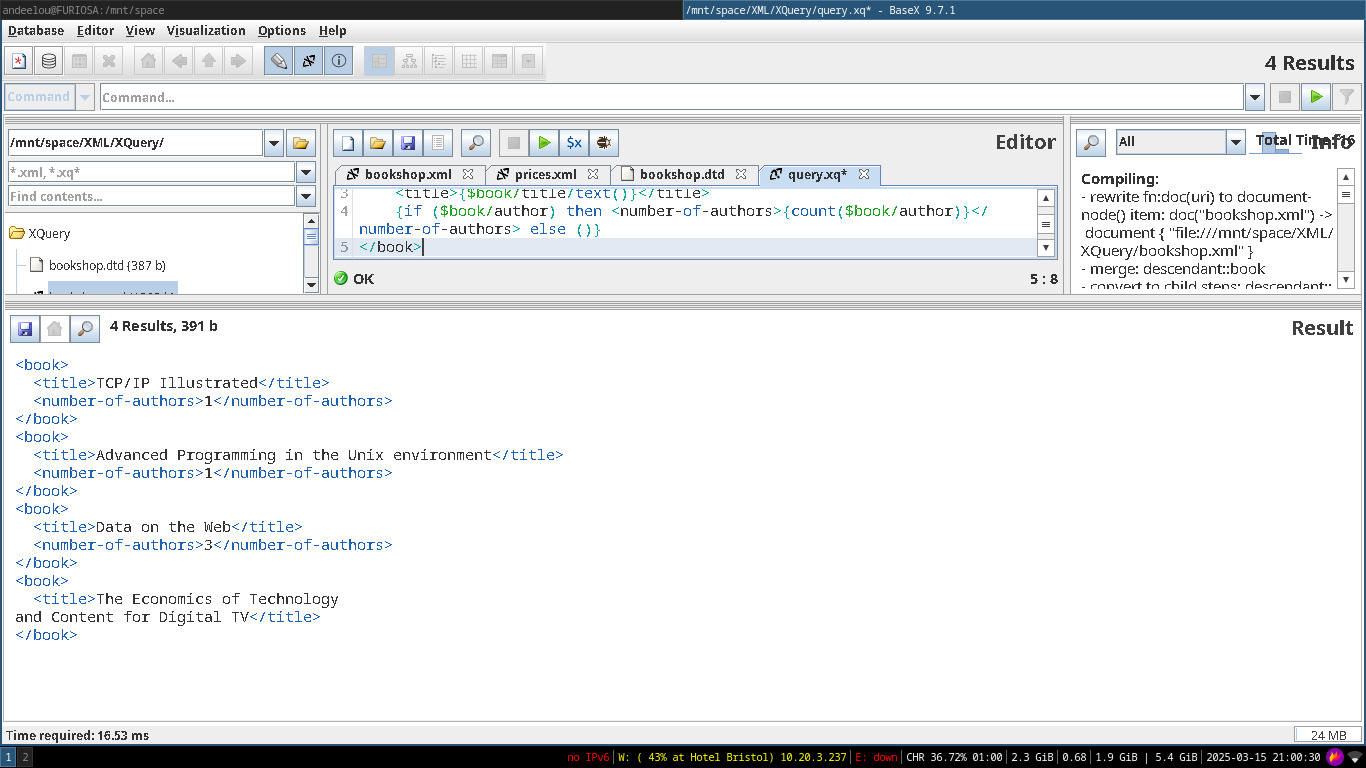
\includegraphics[width=1\textwidth]{imgs/x6.jpeg}
			\caption{Minimum price for each book.}
			\label{fig:6}
			\small{The query calculates the minimum price for each book across different stores.}
		\end{figure}
%7
	\item Alphabetically list Addison-Wesley books after 1991:
		\begin{lstlisting}[style=xquery]
			for $book in doc("bookshop.xml")//book
			where $book/publisher = "Addison-Wesley" and $book/@year > 1991
			order by $book/title
			return <book>
			<title>{$book/title/text()}</title>
			<year>{$book/@year}</year>
			</book>
		\end{lstlisting}
		\subsection*{Query Result}
		\begin{figure}[H]
			\centering
			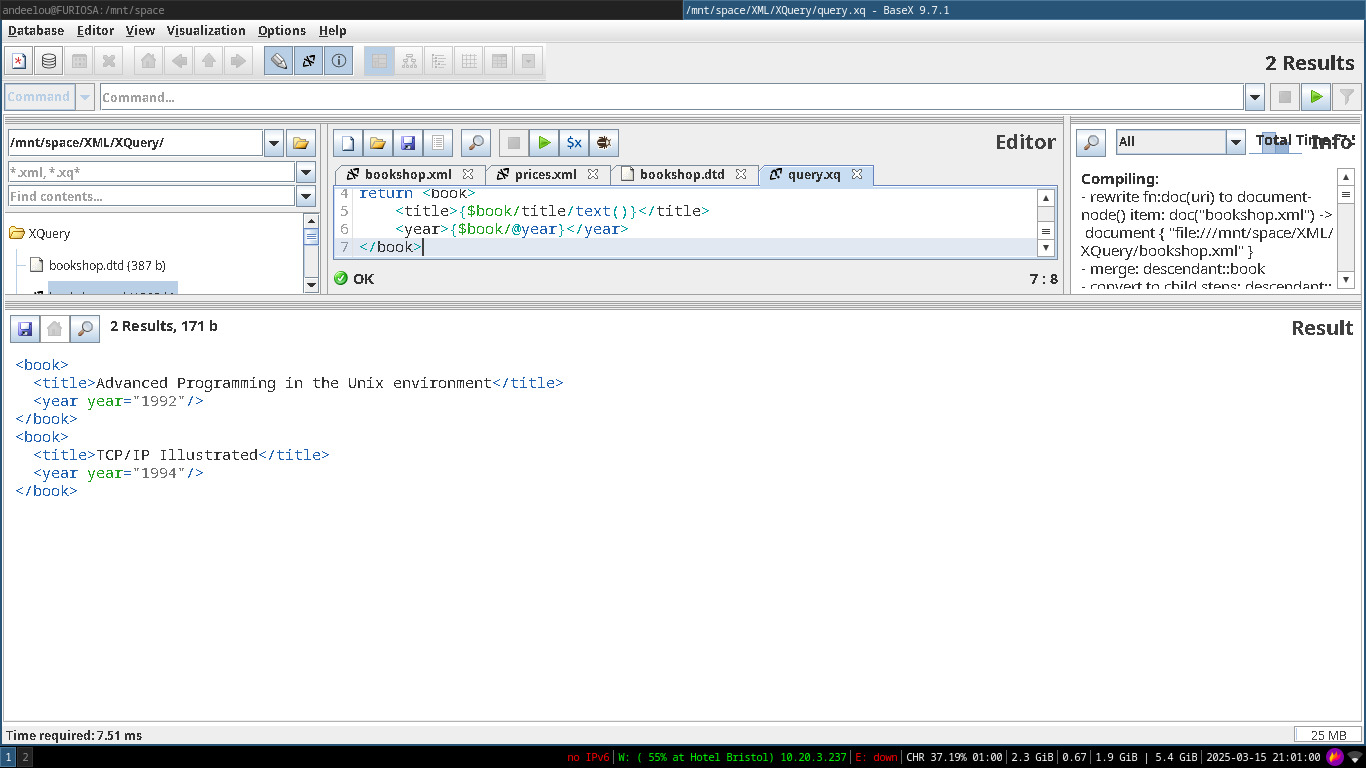
\includegraphics[width=1\textwidth]{imgs/x7.jpeg}
			\caption{Alphabetically listed Addison-Wesley books after 1991.}
			\label{fig:7}
			\small{The query filters and sorts books by title, showing only those published by Addison-Wesley after 1991.}
		\end{figure}
%8
	\item Return book element for authored books, reference for published ones:
		\begin{lstlisting}[style=xquery]
			for $book in doc("bookshop.xml")//book
			return
			if ($book/author)
			then <book>
			<title>{$book/title/text()}</title>
			<authors>{
				for $author in $book/author
				return <author>{$author/name/text()} {$author/lastname/text()}</author>
			}</authors>
			</book>
			else if ($book/editor)
			then <reference>
			<title>{$book/title/text()}</title>
			<affiliation>{$book/editor/affiliation/text()}</affiliation>
			</reference>
			else ()
		\end{lstlisting}
		\subsection*{Query Result}
		\begin{figure}[H]
			\centering
			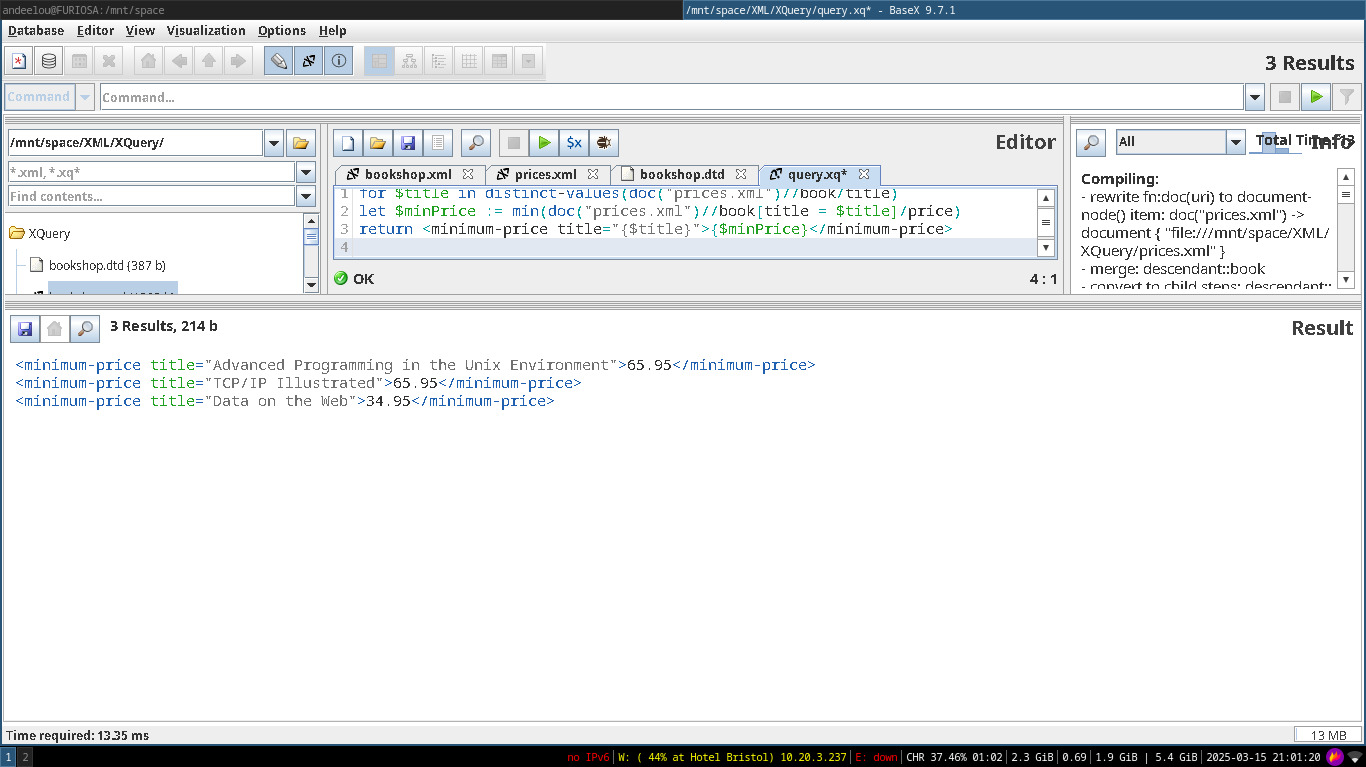
\includegraphics[width=1\textwidth]{imgs/x8.jpeg}
			\caption{Books and references differentiated by author or editor.}
			\label{fig:8}
			\small{The query differentiates between authored books and edited references, returning different XML structures for each.}
		\end{figure}
%9
	\item List book titles with their prices at each bookshop:
		\begin{lstlisting}[style=xquery]
			for $book in distinct-values(doc("prices.xml")//book/title)
			return <book>
			<title>{$book/text()}</title>
			{
				for $store in doc("prices.xml")//book[title = $book]
				return <price source="{$store/source/text()}">{$store/price/text()}</price>
			}
			</book>
		\end{lstlisting}
		\subsection*{Query Result}
		\begin{figure}[H]
			\centering
			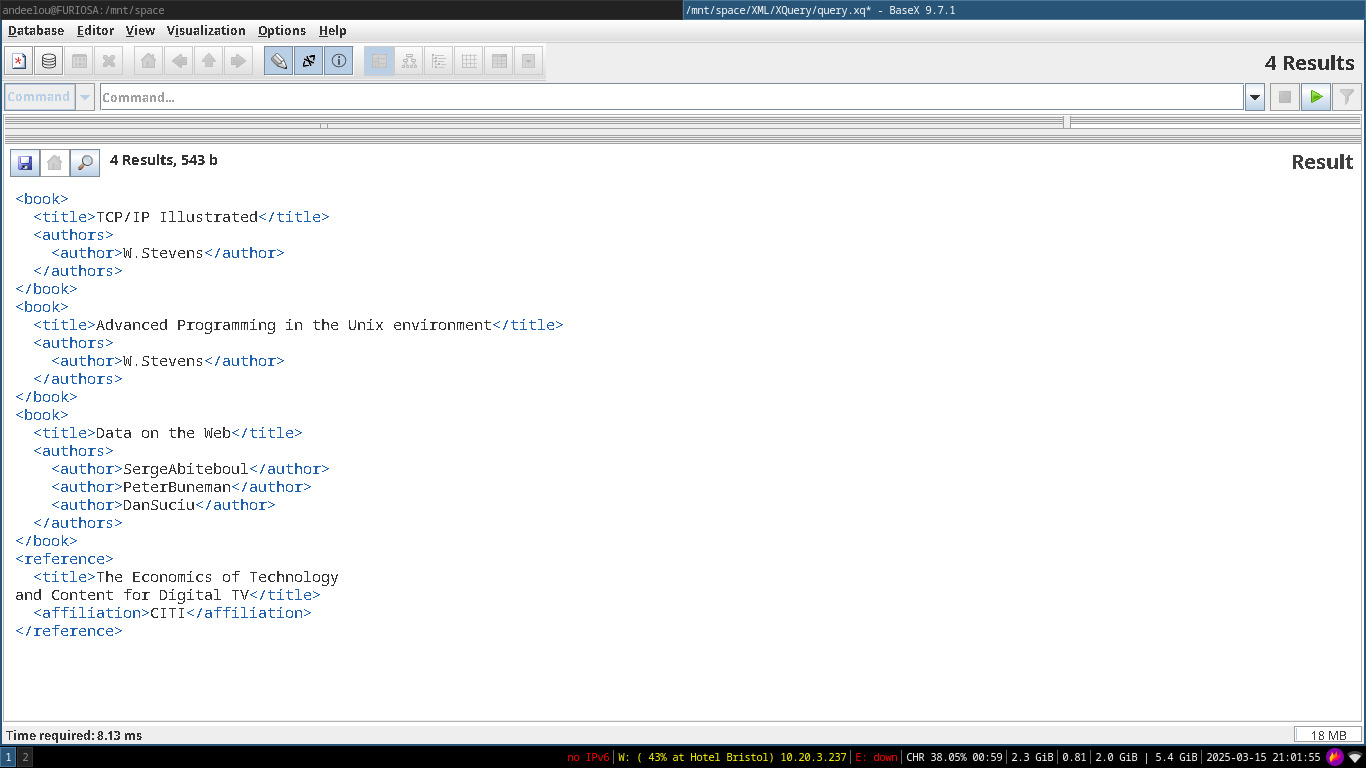
\includegraphics[width=1\textwidth]{imgs/x9.jpeg}
			\caption{Book titles with prices at each bookshop.}
			\label{fig:9}
			\small{The query lists each book title along with its prices from different stores.}
		\end{figure}
\end{enumerate}

\section{Conclusions}
Through this exercise, we gained a deeper understanding of the XQuery language and its capabilities in querying and transforming XML data. The practical examples demonstrated the flexibility and power of XQuery in handling complex data retrieval and manipulation tasks. Future work could explore advanced features such as XQuery functions, modules, and integration with other technologies, will ORACLE save us from a painfull dev experiencie with XML?

\section*{Our Team experiencie with AI on the activity}
We as a team were unable to implement the solutions that the artificial intelligence tried to provide because they still need to mature on archaic technologies, and because this technologies are used in the laboral field, the information of methodologies of using such technologies are not in the range of ChatGPT's or any other AI database.

\begin{thebibliography}{9}
	\bibitem{w3}
	XQuery 3.1: An XML query language. (n.d.). Www.w3.org. Retrieved March 15, 2025, from \url{https://www.w3.org/TR/xquery-31/}
	\bibitem{microsoft}
	XQuery language reference (SQL Server). (n.d.). Microsoft.com. Retrieved March 15, 2025, from \url{https://learn.microsoft.com/en-us/sql/xquery/xquery-language-reference-sql-server?view=sql-server-ver16}
	\bibitem{w3schools}
	XQuery tutorial. (n.d.). W3schools.com. Retrieved March 15, 2025, from \url{https://www.w3schools.com/xml/xquery_intro.asp}
\end{thebibliography}

\end{document}
